\section{Probabilités}
\subsection{Problématique}

	Quelle est la probabilité que les prisonniers survivent ?
	D'un premier instinct, si chaque prisonnier peut ouvrir la moitié des boîtes, alors la probabilité qu'un prisonnier
	trouve son numéro parmi les boîtes qu'il a ouvert est de $\frac{1}{2}$. Donc la probabilité que tous trouvent leur
	numéro respectif est de $$\left(\frac{1}{2}\right)^{100} \approx 0.789 * 10^{-30}$$
	Y a-t-il une méthode qui permettrait de considérablement augmenter ces chances ?

\subsection{Probabilités de cycles}

	Nous avons vu dans la section précédente que le nombre de permutations de $n$ éléments contenant un cycle de longueur $0 < k \leq n$ est de $\frac{n!}{k}$.
	À partir de cette information, nous sommes maintenant en mesure de calculer la probabilité d'obtenir un cycle de longueur $\frac{n}{2} < k \leq n$ dans une permutation de $n$ éléments.
	Nous ne parlerons pas ici de la probabilité qu'il y ait un cycle de longueur $k$ lorsque $0 < k \leq \frac{n}{2}$.

	Soient les événements aléatoires
	\begin{align*}
		E_k  & : "\text{Une permutation de n éléments contient un cycle de longueur k.}"          \\
		E'_k & : "\text{Une permutation de n éléments contient un cycle de longueur au moins k.}"
	\end{align*}

	Muni de la \href{https://fr.wikipedia.org/wiki/Loi_uniforme_discr%C3%A8te#Calcul_d'une_probabilit%C3%A9}{loi uniforme discrète}, on sait que $P(X \in B) = \frac{\#(A \cap B)}{\#A}$, de fait :

	\begin{equation}
		P(E_k) = \frac{\frac{n!}{k}}{n!} = \frac{1}{k}
	\end{equation}

	À partir de $P(E_k)$, on peut désormais aisément calculer $P(E'_k)$ :

	\begin{equation}
		P(E'_k) = \sum_{i = k}^{n} P(E_i) = \sum_{i = k}^{n} \frac{1}{i}
	\end{equation}

	On reconnaît ici une forme de \href{https://en.wikipedia.org/wiki/Harmonic_series_(mathematics)#}{série harmonique}.
	En prenant $k = \frac{n}{2}$, on obtient

	\begin{equation}
		P(E'_{\frac{n}{2}}) = \frac{1}{\frac{n}{2}} + \hdots + \frac{1}{n - 1} + \frac{1}{n}
	\end{equation}

	Il est possible de développer en utilisant la série Harmonique.

	\begin{align*}
		P(E'_{\frac{n}{2}}) & = H(n) - H(\lfloor \frac{n}{2} \rfloor)     \\
		                    & \approx \ln{n} - \ln{\frac{n}{2}}           \\
		                    & \approx \ln{\frac{n}{\frac{n}{2}}} = \ln{2} \\
		                    & \approx 0.693147181
	\end{align*}

	En conclusion, il y a environ 70\% de chances qu'une permutation de $n$ éléments contiennent un cycle d'au moins $\frac{n}{2}$.

\subsection{Interpretation}

	Nous savons que les prisonniers ne peuvent s'en sortir que si le cycle maximal est de $\frac{n}{2}$.
	Ce qui leur laisse environ 30\% de chance de survie.

\subsection{Expérimentation}

\begin{figure}[h]
  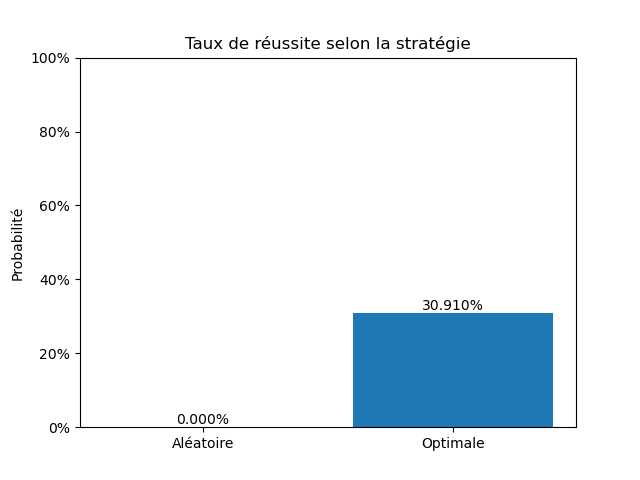
\includegraphics[width=\linewidth]{./strategies_succes.png}
  \caption{Taux de réussite selon la stratégie}
  \label{fig:strategies_success}
\end{figure}

\begin{figure}[h]
  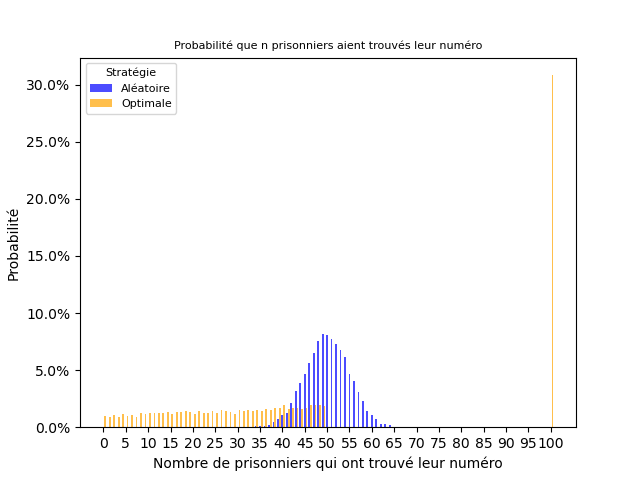
\includegraphics[width=\linewidth]{./strategies_outcomes.png}
  \caption{Probabilité que $n$ prisonniers aient trouvés leur numéro}
  \label{fig:strategies_outcomes}
\end{figure}